%!TEX root = ../../main.tex

\chapter{Experiments} \label{chap:experimental_result}
    \section{Introduction}
        This chapter represents the methodology proposed in this thesis.
        In section \ref{sec:datasets} and section \ref{sec:protocol}, the benchmarking datasets and evaluation protocol used in experiments of this thesis will be listed out.
        Section \ref{sec:experimental_setup} gives details about the programming configurations of the experiments.
        And finally, section \ref{sec:results} shows the experimental outcomes of proposed framework, compares them with results reported in existing publications and gives discussion.

    %!TEX root = ../../../main.tex

\section{Experimental Results and Discussions} \label{sec:results}
    %!TEX root = ../../../main.tex

\subsection{Experimental results on IXMAS dataset}
    \paragraph{1) Cross-view validation:} In this experiment, we train on data from one view (training view) and testing on data from another view (testing view) then compute the accuracies for two evaluation protocols. Table \ref{tab:cross_p1_ixmas} shows comparative results of using different deep features (C3D, ResNet-50 3D, ResNet-50 RNN, ResNet-50 TA, ResNet-50 AP) and multi-view discriminant analysis techniques (MvDA, MvDA-vc and our proposed pc-MvDA). 

    With the first evaluation protocol, the proposed pc-MvDA, when combined with deep features, gives mostly best accuracy for both evaluation protocols. With C3D features, accuracy by pc-MvDA (88.43\%) is 6.6\% higher than MvDA (81.84\%). pc-MvDA is even better than MvDA-vc (2.87\%). pc-MvDA achieved higher accuracy (about 6\% higher) than MvDA and MvDA-vc with ResNet-50 TA and ResNet-50 AP features. In average, pc-MvDA is 3.09\% higher than MvDA and 1.4\% higher than MvDA-vc.
    
    \begin{table}[htbp]
    \centering
    \caption{Cross-view recognition comparison on IXMAS dataset.}
    \resizebox{0.8\textwidth}{!}{
    \begin{tabular}{|l|c|c|c|c|c|c|}
        \hline
        \multirow{2}{*}{Deep features}          & \multicolumn{3}{c|}{Protocol 1}   & \multicolumn{3}{c|}{Protocol 2}           \\ \cline{2-7} 
                                                & MvDA  & MvDA-vc & pc-MvDA         & MvDA  & MvDA-vc        & pc-MvDA          \\ \hline
        \multicolumn{1}{|c|}{C3D}               & 81.84 & 85.56   & \textbf{88.43}  & 96.54 & 99.29          & \textbf{99.98}   \\ \hline
        \multicolumn{1}{|c|}{ResNet-50 3D}      & 91.25 & 92.19   & \textbf{92.89}  & 97.30 & \textbf{99.73} & 99.65            \\ \hline
        \multicolumn{1}{|c|}{ResNet-50 RNN}     & 75.51 & 76.12   & \textbf{76.54}  & 99.99 & 99.71          & \textbf{100}     \\ \hline
        \multicolumn{1}{|c|}{ResNet-50 TA}      & 79.44 & 80.58   & \textbf{82.05}  & 99.33 & 99.34          & \textbf{99.84}   \\ \hline
        \multicolumn{1}{|c|}{ResNet-50 AP}      & 77.00 & 79.04   & \textbf{80.58}  & 99.68 & 99.81          & \textbf{99.92}   \\ \hline
    \end{tabular}}
    \label{tab:cross_p1_ixmas}
    \end{table}

    For the second evaluation protocol, pc-MvDA almost always keeps better performance compared to MvDA and MvDA-vc. The recognition accuracy scores obtained by both pc-MvDA and MvDA-vc are nearly 100\% for every kind of deep features. With C3D features and ResNet-50 3D features, pc-MvDA is 99.98\% and 99.65\%, which is 3.44\% and 2.35\% higher than the orginal MvDA (96.54\% and 97.3\%) respectively. In average, pc-MvDA is 1.31\% better than MvDA and 0.3\% better than MvDA-vc. 

    In terms of deep features, with the first evaluation protocol, ResNet-50 3D gives the best accuracy (92.89\%) following by C3D (88.43\%), ResNet-50 TA (82.05\%), ResNet-50 AP (80.58\%). The lowest accuracy obtained by ResNet-50 RNN is only 76.54\%. It shows that ResNet-50 3D produces the most discriminative feature space. %Table \ref{tab:cross_feature_ixmas} shows comparative results when using pc-MvDA method with different deep features regarding pairwise views. 

    \begin{table}[htbp]
    \centering
    \caption{Cross-view recognition results of different features on IXMAS dataset with pc-MvDA method. The result in the bracket are accuracies of using features C3D, ResNet-50 3D, ResNet-50 RNN, ResNet-50 TA, Restnet-50 AP respectively. Each row corresponds to training view (from view C0 to view C3). Each column corresponds to testing view (from view C0 to view C3).}
    \resizebox{\textwidth}{!}{\begin{tabular}{|c|c|c|c|c|}
        \hline
        \backslashbox{Training}{Testing} & C0 & C1 & C2 & C3 \\ \hline
        C0 & N/A & (90.7, \textbf{91.9}, 81.6, 84.6, 83.6) & (86.9, \textbf{93.9}, 78.0, 79.6, 78.1) & (89.9, \textbf{93.4}, 76.3, 82.8, 82.1) \\ \hline
        C1 & (86.6, \textbf{91.9}, 71.5, 81.1, 77.5) & N/A & (85.9, \textbf{94.2}, 78.6, 79.3, 80.3) & (88.9, \textbf{93.7}, 74.8, 82.3, 81.3) \\ \hline
        C2 & (87.6, \textbf{92.4}, 72.8, 81.8, 78.5) & (90.7, \textbf{91.7}, 80.6, 83.6, 82.6) & N/A & (89.4, \textbf{93.7}, 75.5, 82.3, 80.6) \\ \hline
        C3 & (87.6, \textbf{92.9}, 70.2, 82.1, 78.8) & (90.7, \textbf{91.2}, 81.6, 84.1, 82.8) & (86.4, \textbf{93.7}, 77.3, 80.6, 80.8) & N/A \\ \hline
    \end{tabular}}
    \label{tab:cross_feature_ixmas}
    \end{table}

    \paragraph{2) Multi-view validation} Table \ref{tab:ixmas_multi} shows multi-view recognition results. The conclusion is consistent with the case of cross-view evaluation: ResNet-50 3D is the best feature extractor. When it is combined with pc-MvDA, the framework gives the highest accuracy for the first protocol (92.82\%), following by C3D (88.19\%), ResNet-50 TA (81.49\%), ResNet-50 AP(80.43\%), and ResNet-50 RNN (76.47\%). Both MvA algorithms give similar accuracies for the second evaluation protocols (nearly 100\%). Again, pc-MvDA enhances the performance of MvDA by 2.43\% for the first protocol and 0.83\% for the second protocol. It only gives slightly better result than MvDA-vc (0.83\% for the first protocol and 0.74\% for the second protocol). 

    \begin{table}[htbp]
    \centering
    \caption{Multi-view recognition comparison on IXMAS dataset.}
    \resizebox{0.7\textwidth}{!}{\begin{tabular}{|c|c|c|c|c|c|c|}
        \hline
        \multirow{2}{*}{Deep features}          & \multicolumn{3}{c|}{Protocol 1}   & \multicolumn{3}{c|}{Protocol2}                    \\ \cline{2-7} 
                                                & MvDA  & MvDA-vc & pc-MvDA         & MvDA           & MvDA-vc        & pc-MvDA         \\ \hline
        \multicolumn{1}{|c|}{C3D}               & 86.93 & 87.04   & \textbf{88.19}  & \textbf{99.99} & 99.44          & \textbf{99.98}  \\ \hline
        \multicolumn{1}{|c|}{ResNet-50 3D}      & 91.84 & 92.33   & \textbf{92.82}  & \textbf{100}   & 99.80          & 99,67           \\ \hline
        \multicolumn{1}{|c|}{ResNet-50 RNN}     & 72.44 & 75.95   & \textbf{76.47}  & 99.34          & \textbf{99.97} & \textbf{99.96}  \\ \hline
        \multicolumn{1}{|c|}{ResNet-50 TA}      & 76.74 & 81.01   & \textbf{81.49}  & 95.80          & 98.25          & \textbf{99.79}  \\ \hline
        \multicolumn{1}{|c|}{ResNet-50 AP}      & 79.28 & 78.93   & \textbf{80.43}  & \textbf{100}   & 98.11          & 99.85           \\ \hline
    \end{tabular}}
    \label{tab:ixmas_multi}
    \end{table}

    Figure \ref{fig:pc-MvDA_confusion_ixmas} compares the performance of feature extractors regarding each action class in multi-view evaluation scheme combined with the first evaluation protocol. There are clear margins between the performance of ResNet-50 3D and followed by C3D with other types of deep features, especially in harder actions (the first class to the third class and the eighth class to the eleventh class). These actions (check watch, cross arm, scratch head, wave, punch, kick, point) involve the most part static pose of the body and only movement of limbs, whereas other actions 4 - sit down, 5 - get up, 6 - turn around, 7 - walk and 12 - pickup include movement of the whole body and are easier to be recognized. This suggests that 3D convolution can better deal with small difference of movement in action images, which in turn generates a much more classification-ready feature space for latter stage of recognition.

    \begin{figure}[htbp]
        \centering
        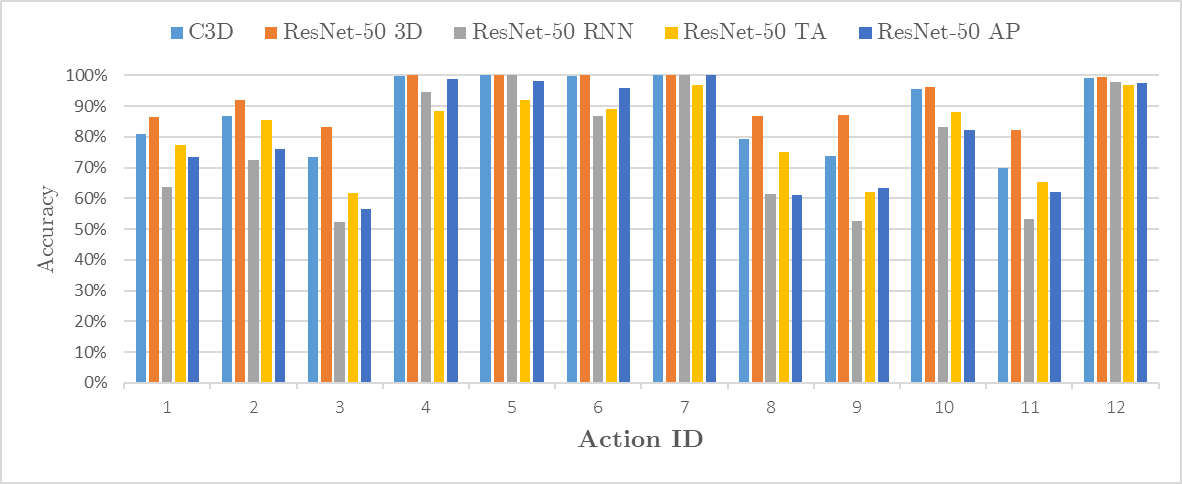
\includegraphics[width=0.8\linewidth]{figs/pc-MvDA_confusion_ixmas.png}
        \caption{Comparison of accuracy on each action class using different deep features combined with pc-MvDA on IXMAS dataset.}
        %\vspace{-0.3cm}
        \label{fig:pc-MvDA_confusion_ixmas}
    \end{figure}

    Table \ref{tab:sota_ixmas} compares the best combination of ResNet-50 3D and pc-MvDA with state-of-the-art frameworks. The comparison is for reference only because in other works, low-level hand-crafted video representation is used as private features and train-test strategy is leave-one-class out, which is not applicable to supervised deep feature extractors in this work. However, the results are still commensurable. % in circumstances where supervised approaches are adopted.
    % TODO - High priority

    \begin{table}[htbp]
    \centering
    \caption{Comparison of proposed methods with SOTA methods on IXMAS dataset according to the second evaluation protocol.}
    \resizebox{0.7\textwidth}{!}{
    \begin{tabular}{|c|c|c|}
    \hline
    Methods                                                              & Cross-view & Multi-view \\ \hline
    Liu et al. \cite{liu2011cross}                                   & 76.32      & N/A       \\ \hline
    Zheng et al. \cite{zheng2012cross}                               & 95.1       & 99.32     \\ \hline
    Zheng et al. \cite{zheng2016cross}                               & 97.8       & 99.4      \\ \hline
    Kong et al. \cite{kong2017deeply}                                & 99.92      & 100       \\ \hline
    Ulhaq et al. \cite{ulhaq2017space}                               & 66.82      & 92.47     \\ \hline
    Zhang et al. \cite{zhang2018cross}                               & 84.1       & N/A        \\ \hline
    Liu et al. \cite{liu2018learning}                                & N/A        & 90.3     \\ \hline
    Liu et al. \cite{liu2018hierarchically}                          & 99.95      & 99.67     \\ \hline
    Proposed method (ResNet-50 3D + pc-MvDA)                     & 99.67      & 99.65       \\ \hline
    \end{tabular}}
    \label{tab:sota_ixmas}
    \end{table}

    %!TEX root = ../../../main.tex

\subsection{Experimental results on MuHAVi dataset}
    \paragraph{1) Cross-view validation:} Table.\ref{tab:muhavi_cross} illustrates cross-view recognition results. The proposed pc-MvDA consistently produces a better average accuracy of around 96.19\% for protocol 1, approximately 4.55\% and 1.51\% higher than that of MvDA (91.64\%) and MvDA-vc (94.67\%) respectively.

    \begin{table}[htbp]
    \centering
    \caption{Cross-view recognition comparison on MuHAVi dataset.}
    \resizebox{0.8\textwidth}{!}{
    \begin{tabular}{|c|c|c|c|c|c|c|}
        \hline
        \multirow{2}{*}{Deep features}          & \multicolumn{3}{c|}{Protocol 1}   & \multicolumn{3}{c|}{Protocol 2}           \\ \cline{2-7} 
                                                & MvDA  & MvDA-vc & pc-MvDA         & MvDA  & MvDA-vc        & pc-MvDA          \\ \hline
        \multicolumn{1}{|c|}{C3D}               & 92.85 & 95.15   & \textbf{97.65}  & 98.95 & 99.76          & \textbf{100}     \\ \hline
        \multicolumn{1}{|c|}{ResNet-50 3D}      & 97.94 & 99.15   & \textbf{99.18}  & 96.77 & \textbf{99.94} & \textbf{99.94}   \\ \hline
        \multicolumn{1}{|c|}{ResNet-50 RNN}     & 95.54 & 95.14   & \textbf{96.18}  & 98.70 & 99.05          & \textbf{99.99}   \\ \hline
        \multicolumn{1}{|c|}{ResNet-50 TA}      & 85.80 & 88.95   & \textbf{91.12}  & 96.57 & 97.03          & \textbf{99.88}   \\ \hline
        \multicolumn{1}{|c|}{ResNet-50 AP}      & 86.09 & 94.98   & \textbf{96.82}  & 89.04 & 98.62          & \textbf{99.93}   \\ \hline
    \end{tabular}}
    \label{tab:muhavi_cross}
    \end{table}

    %Results in Table.\ref{tab:cross_feature_muhavi} show that our combination with ResNet-50 3D has the highest accuracies in almost every circumstances, even though both features coupled with our proposed pc-MvDA give satisfactory performance with all scores exceeding 91\%.

    \begin{table}[htbp]
    \centering
    \caption{Cross-view recognition results of different features on MuHAVi dataset with pc-MvDA method. The result in the bracket are accuracies of using features C3D, ResNet-50 3D, ResNet-50 RNN, ResNet-50 TA, ResNet-50 AP respectively. Each row corresponds to training view (from view C1 to view C7). Each column corresponds to testing view (from view C1 to view C7).}
    \resizebox{\textwidth}{!}{\begin{tabular}{|c|c|c|c|c|c|c|c|}
        \hline
        \backslashbox{Training}{Testing} & C1 & C2 & C3 & C4 & C5 & C6 & C7 \\ \hline
        C1 & N/A & \begin{tabular}{@{}c@{}} (96.1, \textbf{100}, 96.8, \\ 88.5, 98.5) \end{tabular} & \begin{tabular}{@{}c@{}} (98.6, \textbf{99.6}, 96.6, \\ 88.9, 96.3) \end{tabular} & \begin{tabular}{@{}c@{}} (98.6, \textbf{99.6}, 98.0, \\ 93.1, 98.2) \end{tabular} & \begin{tabular}{@{}c@{}} (97.7, \textbf{99.6}, 95.4, \\ 91.3, 96.1) \end{tabular} & \begin{tabular}{@{}c@{}} (97.7, \textbf{98.4}, 92.3, \\ 93.1, 96.3) \end{tabular} & \begin{tabular}{@{}c@{}} (98.2, \textbf{98.5}, 97.2, \\ 89.8, 97.1) \end{tabular} \\ \hline
        C2 & \begin{tabular}{@{}c@{}} (95.6, \textbf{99.0}, 95.2, \\ 91.3, 95.5) \end{tabular} & N/A & \begin{tabular}{@{}c@{}} (98.9, \textbf{99.6}, 96.9, \\ 90.3, 96.1) \end{tabular} & \begin{tabular}{@{}c@{}} (98.4, \textbf{99.6}, 97.6, \\ 92.6, 98.2) \end{tabular} & \begin{tabular}{@{}c@{}} (97.7, \textbf{99.6}, 95.4, \\ 90.9, 96.1) \end{tabular} & \begin{tabular}{@{}c@{}} (97.8, \textbf{98.4}, 92.7, \\ 93.6, 96.5) \end{tabular} & \begin{tabular}{@{}c@{}} (98.6, \textbf{99.0}, 97.4, \\ 90.6, 96.9) \end{tabular} \\ \hline
        C3 & \begin{tabular}{@{}c@{}} (96.1, \textbf{99.0}, 95.6, \\ 90.3, 95.1) \end{tabular} & \begin{tabular}{@{}c@{}} (97.0, \textbf{100}, 96.7, \\ 88.4, 97.8) \end{tabular} & N/A & \begin{tabular}{@{}c@{}} (98.1, \textbf{99.2}, 98.2, \\ 92.8, 98.2) \end{tabular} & \begin{tabular}{@{}c@{}} (97.9, \textbf{99.6}, 95.4, \\ 90.2, 95.6) \end{tabular} & \begin{tabular}{@{}c@{}} (97.9, \textbf{98.2}, 93.0, \\ 94.2, 96.5) \end{tabular} & \begin{tabular}{@{}c@{}} (97.8, \textbf{98.7}, 97.4, \\ 89.4, 97.6) \end{tabular} \\ \hline
        C4 & \begin{tabular}{@{}c@{}} (96.4, \textbf{98.8}, 95.4, \\ 89.6, 95.3) \end{tabular} & \begin{tabular}{@{}c@{}} (96.3, \textbf{100}, 96.6, \\ 91.0, 98.5) \end{tabular} & \begin{tabular}{@{}c@{}} (98.6, \textbf{99.6}, 97.3, \\ 89.5, 96.1) \end{tabular} & N/A & \begin{tabular}{@{}c@{}} (97.7, \textbf{99.4}, 95.6, \\ 91.3, 96.1) \end{tabular} & \begin{tabular}{@{}c@{}} (\textbf{98.4}, 98.0, 93.2, \\ 93.8, 95.6) \end{tabular} & \begin{tabular}{@{}c@{}} (97.7, \textbf{98.7}, 97.4, \\ 91.3, 96.7) \end{tabular} \\ \hline
        C5 & \begin{tabular}{@{}c@{}} (95.9, \textbf{99.0}, 95.6, \\ 91.3, 95.5) \end{tabular} & \begin{tabular}{@{}c@{}} (96.6, \textbf{100}, 97.1, \\ 89.9, 98.3) \end{tabular} & \begin{tabular}{@{}c@{}} (98.8, \textbf{99.4}, 96.8, \\ 90.7, 96.1) \end{tabular} & \begin{tabular}{@{}c@{}} (98.4, \textbf{99.6}, 98.0, \\ 92.1, 97.6) \end{tabular} & N/A & \begin{tabular}{@{}c@{}} (97.9, \textbf{98.2}, 93.4, \\ 94.4, 96.8) \end{tabular} & \begin{tabular}{@{}c@{}} (98.0, \textbf{98.7}, 96.9, \\ 89.0, 97.8) \end{tabular} \\ \hline
        C6 & \begin{tabular}{@{}c@{}} (95.8, \textbf{99.0}, 95.8, \\ 90.3, 95.0) \end{tabular} & \begin{tabular}{@{}c@{}} (97.0, \textbf{100}, 97.6, \\ 89.7, 98.5) \end{tabular} & \begin{tabular}{@{}c@{}} (98.8, \textbf{99.6}, 96.9, \\ 88.7, 96.1) \end{tabular} & \begin{tabular}{@{}c@{}} (98.4, \textbf{99.4}, 98.0, \\ 92.8, 98.2) \end{tabular} & \begin{tabular}{@{}c@{}} (97.5, \textbf{99.6}, 95.9, \\ 91.2, 95.5) \end{tabular} & N/A & \begin{tabular}{@{}c@{}} (98.2, \textbf{99.0}, 97.2, \\ 90.7, 97.4) \end{tabular} \\ \hline
        C7 & \begin{tabular}{@{}c@{}} (96.2, \textbf{98.8}, 95.7, \\ 91.5, 96.2) \end{tabular} & \begin{tabular}{@{}c@{}} (96.4, \textbf{100}, 97.5, \\ 90.3, 98.5) \end{tabular} & \begin{tabular}{@{}c@{}} (98.4, \textbf{99.0}, 97.3, \\ 90.0, 96.7) \end{tabular} & \begin{tabular}{@{}c@{}} (\textbf{98.8}, 98.8, 98.2, \\ 92.8, 98.0) \end{tabular} & \begin{tabular}{@{}c@{}} (97.5, \textbf{99.8}, 95.9, \\ 91.5, 95.9) \end{tabular} & \begin{tabular}{@{}c@{}} (\textbf{98.9}, 98.2, 92.8, \\ 93.9, 97.1) \end{tabular} & N/A \\ \hline
    \end{tabular}}
    \label{tab:cross_feature_muhavi}
    \end{table}

    \paragraph{2) Multi-view validation}: Table.\ref{tab:muhavi_multi} shows multi-view recognition results. The first protocol shows very close capability of MvDA-vc and pc-MvDA at 95.54\% and 95.83\% whereas MvDA is about 3\% behind at 92.7\%. For the second protocol, our variant exceeds MvDA by 2.21\% and MvDA-vc by 1.49\%. The near perfect results of the second protocol give us the same indication that it is not an inequitable method of comparison of MvA algorithms. 

    \begin{table}[htbp]
    \centering
    \caption{Multi-view recognition comparison on MuHAVi dataset.}
    \resizebox{0.8\textwidth}{!}{
    \begin{tabular}{|c|c|c|c|c|c|c|}
        \hline
        \multirow{2}{*}{Deep features}          & \multicolumn{3}{c|}{Protocol 1}                   & \multicolumn{3}{c|}{Protocol2}            \\ \cline{2-7} 
                                                & MvDA           & MvDA-vc        & pc-MvDA         & MvDA           & MvDA-vc & pc-MvDA        \\ \hline
        \multicolumn{1}{|c|}{C3D}               & 81.80          & 96.05          & \textbf{97.37}  & 88.39          & 99.61   & \textbf{100}   \\ \hline
        \multicolumn{1}{|c|}{ResNet-50 3D}      & 99.07          & 99.12          & \textbf{99.15}  & \textbf{99.98} & 99.96   & 99.89          \\ \hline
        \multicolumn{1}{|c|}{ResNet-50 RNN}     & \textbf{96.18} & 95.55          & 95.97           & \textbf{100}   & 99.00   & 99.98          \\ \hline
        \multicolumn{1}{|c|}{ResNet-50 TA}      & \textbf{90.45} & 89.73          & 90.22           & \textbf{99.92} & 98.17   & 99.72          \\ \hline
        \multicolumn{1}{|c|}{ResNet-50 AP}      & 96.01          & \textbf{96.75} & 96.42           & \textbf{100}   & 95.13   & 99.68          \\ \hline
    \end{tabular}}
    \label{tab:muhavi_multi}
    \end{table}

    Figure \ref{fig:pc-MvDA_confusion_muhavi} compares the performance of feature extractors regarding each action class in multi-view evaluation scheme combined with protocol 1. For this dataset, ResNet-50 3D persistently yields out-standing performance while ResNet-50 TA has the worst recognition rates in all action classes.

    \begin{figure}[htbp]
        \centering
        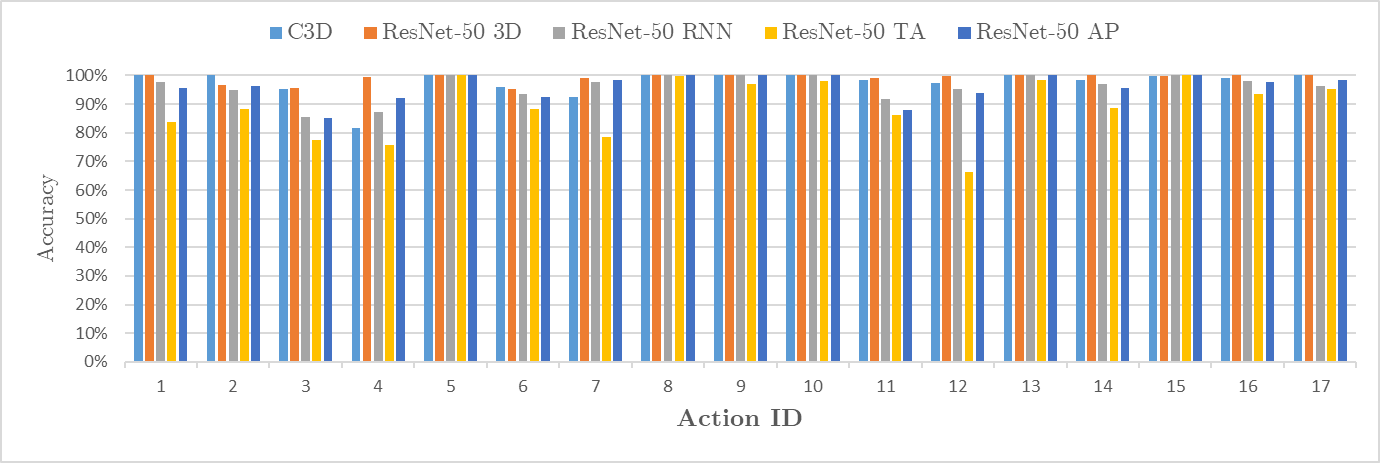
\includegraphics[width=1.0\linewidth]{figs/pc-MvDA_confusion_muhavi.png}
        \caption{Comparison of accuracy on each action class using different deep features combined with pc-MvDA.}
        %\vspace{-0.3cm}
        \label{fig:pc-MvDA_confusion_muhavi}
    \end{figure}

    Table \ref{tab:sota_muhavi} compares the best investigated combination of ResNet-50 3D and pc-MvDA with state-of-the-art frameworks. The comparison is for reference only because of aforementioned difference in setup of number of views and cross validation scheme.

    \begin{table}[htbp]
    \centering
    \caption{Comparison of the proposed methods with SOTA methods on MuHAVi dataset according to the second evaluation protocol.}
    \resizebox{0.7\textwidth}{!}{
    \begin{tabular}{|c|c|c|}
    \hline
    Methods                                                   & Cross-view & Multi-view \\ \hline
    Wu et al. \cite{wu2012view}                               & N/A       & 94.5     \\ \hline
    Zheng et al. \cite{zheng2016cross}                        & 94.88     & 99.8     \\ \hline
    Liu et al. \cite{liu2018learning}                         & N/A       & 91.2     \\ \hline
    Liu et al. \cite{liu2018hierarchically}                   & 99.91     & 99.8     \\ \hline
    Proposed method (ResNet-50 3D + pc-MvDA) \protect\footnotemark              & 99.90     & 99.88    \\ \hline
    \end{tabular}}
    \label{tab:sota_muhavi}
    \end{table}
    \footnotetext{Results when choosing only 4 views Camera 1, Camera 3, Camera 4 and Camera 6 following the other works.}

    %!TEX root = ../../../main.tex

\subsection{Experimental results on MICAGes dataset}

    \paragraph{1) Cross-view validation:} It can be seen in Table.\ref{tab:mica_cross} that pc-MvDA outperforms in almost every cases. With the first protocol, the norm accuracy of pc-MvDA of 74.52\% surpasses that of MvDA-vc (72.12\%) by 2.4\% and that of MvDA (64.94\%) by a large margin of 9.58\%. Especially in case of C3D features, the proposed algorithm achieved 90.2\% recognition rate whereas MvDA returns only 67.13\%.

    \begin{table}[htbp]
    \centering
    \caption{Cross-view recognition comparison on MICAGes dataset.}
    \resizebox{0.8\textwidth}{!}{
    \begin{tabular}{|c|c|c|c|c|c|c|}
        \hline
        \multirow{2}{*}{Deep features}          & \multicolumn{3}{c|}{Protocol 1}          & \multicolumn{3}{c|}{Protocol 2}            \\ \cline{2-7} 
                                                & MvDA  & MvDA-vc        & pc-MvDA         & MvDA  & MvDA-vc        & pc-MvDA           \\ \hline
        \multicolumn{1}{|c|}{C3D}               & 67.13 & 85.98          & \textbf{90.20}  & 93.74 & 99.80          & \textbf{100}      \\ \hline
        \multicolumn{1}{|c|}{ResNet-50 3D}      & 94.91 & 95.25          & \textbf{95.62}  & 97.43 & \textbf{99.97} & 99.79             \\ \hline
        \multicolumn{1}{|c|}{ResNet-50 RNN}     & 58.01 & 61.64          & \textbf{64.13}  & 100   & 100            & 100               \\ \hline
        \multicolumn{1}{|c|}{ResNet-50 TA}      & 53.58 & \textbf{59.55} & 58.62           & 96.70 & 99.48          & \textbf{99.83}    \\ \hline
        \multicolumn{1}{|c|}{ResNet-50 AP}      & 51.07 & 58.19          & \textbf{64.04}  & 99.73 & \textbf{99.99} & 99.89             \\ \hline
    \end{tabular}}
    \label{tab:mica_cross}
    \end{table}

    %Table.\ref{tab:cross_feature_mica} compares all types of deep features regarding accuracy of the proposed algorithm. 
    The top ranking of features applies identically and radically proves the superiority of 3D convolution based clip-level feature extraction in video recognition: ResNet-50 3D at 95.62\% and C3D at 90.2\%. The rest are ResNet-50 RNN (64.13\%), ResNet-50 AP (64.04\%) and ResNet-50 TA (58.62\%). For the second protocol, MvDA-vc (99.85\%) and pc-MvDA (99.9\%) are nearly even in performance while MvDA achieved 97.52\%.

    \begin{table}[htbp]
    \centering
    \caption{Cross-view recognition results of different features on MICAGes dataset with pc-MvDA method. The result in the bracket are accuracies of using features C3D, ResNet-50 3D, ResNet-50 RNN, ResNet-50 TA, RestNet-50 AP respectively. Each row corresponds to training view (from view K1 to view K5). Each column corresponds to testing view (from view K1 to view K5).}
    \resizebox{\textwidth}{!}{\begin{tabular}{|c|c|c|c|c|c|}
        \hline
        \backslashbox{Training}{Testing} & K1 & K2 & K3 & K4 & K5 \\ \hline
        K1 & N/A & \begin{tabular}{@{}c@{}} (92.9, \textbf{95.5}, 69.4, \\ 63.9, 65.1) \end{tabular} & \begin{tabular}{@{}c@{}} (93.7, \textbf{98.0}, 79.1, \\ 75.8, 74.7) \end{tabular} & \begin{tabular}{@{}c@{}} (90.5, \textbf{97.6}, 64.5, \\ 68.8, 70.8) \end{tabular} & \begin{tabular}{@{}c@{}} (89.2, \textbf{92.6}, 56.0, \\ 43.7, 58.2) \end{tabular} \\ \hline       
        K2 & \begin{tabular}{@{}c@{}} (84.7, \textbf{94.6}, 51.3, \\ 41.4, 53.7) \end{tabular} & N/A & \begin{tabular}{@{}c@{}} (94.6, \textbf{97.6}, 78.9, \\ 75.4, 77.5) \end{tabular} & \begin{tabular}{@{}c@{}} (91.3, \textbf{97.6}, 64.4, \\ 68.5, 68.0) \end{tabular} & \begin{tabular}{@{}c@{}} (87.4, \textbf{92.7}, 56.1, \\ 42.0, 55.6) \end{tabular} \\ \hline       
        K3 & \begin{tabular}{@{}c@{}} (87.5, \textbf{94.9}, 51.9, \\ 43.6, 52.7) \end{tabular} & \begin{tabular}{@{}c@{}} (93.0, \textbf{95.5}, 70.1, \\ 64.7, 63.4) \end{tabular} & N/A & \begin{tabular}{@{}c@{}} (90.0, \textbf{97.6}, 63.2, \\ 62.6, 67.5) \end{tabular} & \begin{tabular}{@{}c@{}} (88.9, \textbf{92.2}, 57.2, \\ 41.8, 56.6) \end{tabular} \\ \hline       
        K4 & \begin{tabular}{@{}c@{}} (86.7, \textbf{94.7}, 50.8, \\ 48.9, 54.9) \end{tabular} & \begin{tabular}{@{}c@{}} (90.2, \textbf{95.5}, 71.5, \\ 68.2, 61.8) \end{tabular} & \begin{tabular}{@{}c@{}} (92.5, \textbf{98.0}, 81.0, \\ 76.0, 74.4) \end{tabular} & N/A & \begin{tabular}{@{}c@{}} (89.7, \textbf{92.3}, 54.3, \\ 44.9, 56.6) \end{tabular} \\ \hline       
        K5 & \begin{tabular}{@{}c@{}} (84.9, \textbf{94.9}, 48.4, \\ 41.5, 57.9) \end{tabular} & \begin{tabular}{@{}c@{}} (90.4, \textbf{95.5}, 72.6, \\ 64.1, 65.7) \end{tabular} & \begin{tabular}{@{}c@{}} (94.0, \textbf{97.8}, 79.1, \\ 72.5, 76.3) \end{tabular} & \begin{tabular}{@{}c@{}} (91.9, \textbf{97.3}, 62.7, \\ 64.1, 69.0) \end{tabular} & N/A \\ \hline
    \end{tabular}}
    \label{tab:cross_feature_mica}
    \end{table}

    \paragraph{2) Multi-view validation}: The multi-view recognition results in Table.\ref{tab:mica_multi} shows an almost alike trend for both protocols. In general, pc-MvDA is 8.95\% and 0.72\% higher in accuracy for protocol 1, and 2.75\% and 0.04\% for protocol 2, in comparison with MvDA and MvDA-pc respectively.

    % TODO
    In virtually every experiments of MICAGes and two earlier benchmark datasets, the proposed extension is superior. The average accuracies of pc-MvDA is, in comparison on protocol 1 (and protocol 2 resp.), 5.29\% (1.21\% resp.) higher than MvDA, 1.21\% (0.62\% resp.) better than MvDA-vc. Despite not being as intuitive and straightly intelligible as pairwise-covariance, the multi-view resemblance added in MvDA-vc achieved nearly the performance of pc-MvDA. However, this view-consistency can be easily splitted into pairwise terms and intergrated into the objective of pc-MvDA in future works for further analysis.

    \begin{table}[htbp]
    \centering
    \caption{Multi-view recognition comparison on MICAGes dataset.}
    \resizebox{0.8\textwidth}{!}{
    \begin{tabular}{|c|c|c|c|c|c|c|}
        \hline
        \multirow{2}{*}{Deep features}          & \multicolumn{3}{c|}{Protocol 1}          & \multicolumn{3}{c|}{Protocol2}                     \\ \cline{2-7} 
                                                & MvDA  & MvDA-vc        & pc-MvDA         & MvDA           & MvDA-vc       & pc-MvDA           \\ \hline
        \multicolumn{1}{|c|}{C3D}               & 68.31 & 87.70          & \textbf{89.99}  & 88.79          & 99.54         & \textbf{100}      \\ \hline
        \multicolumn{1}{|c|}{ResNet-50 3D}      & 95.32 & 95.26          & \textbf{95.54}  & \textbf{100}   & 99.96         & 99.80             \\ \hline
        \multicolumn{1}{|c|}{ResNet-50 RNN}     & 57.50 & 63.05          & \textbf{63.83}  & 99.90          & \textbf{100}  & 99.97             \\ \hline
        \multicolumn{1}{|c|}{ResNet-50 TA}      & 54.43 & \textbf{61.46} & 58.25           & 96.72          & 99.49         & \textbf{99.69}    \\ \hline
        \multicolumn{1}{|c|}{ResNet-50 AP}      & 50.93 & 60.20          & \textbf{63.66}  & \textbf{99.99} & 99.93         & 99.67             \\ \hline
    \end{tabular}}
    \label{tab:mica_multi}
    \end{table}

    In addition to the same propensity shown, MICAGes also reveals the robustness of 3D convolution to generate fine clustered private feature space because this dataset contains exclusively hand gestures, which take part in a relatively small region of the captured videos. ResNet-50 3D and C3D are predominant for discriminant common space construction and classification and distances other features (Figure \ref{fig:pc-MvDA_confusion_mica}).

    \begin{figure}[htbp]
        \centering
        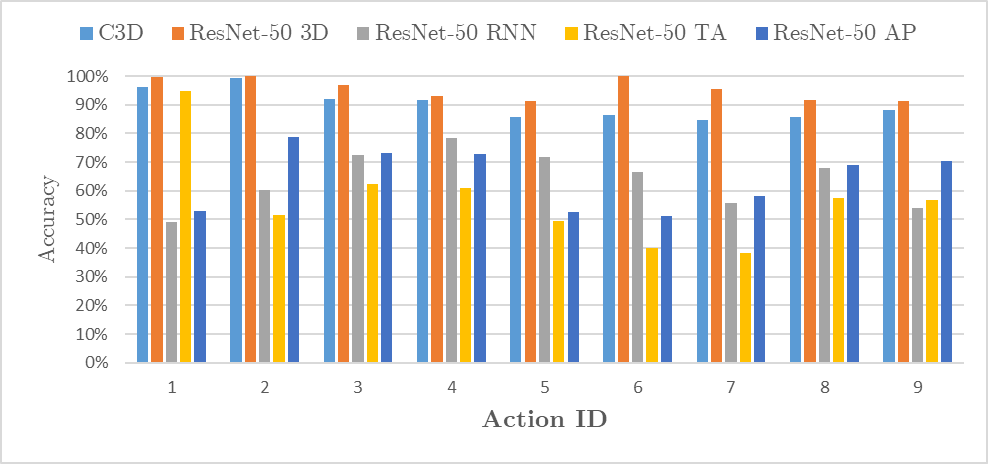
\includegraphics[width=0.8\linewidth]{figs/pc-MvDA_confusion_mica.png}
        \caption{Comparison of accuracy on each action class using different deep features combined with pc-MvDA on MICAGes dataset.}
        %\vspace{-0.3cm}
        \label{fig:pc-MvDA_confusion_mica}
    \end{figure}

    To better study the behavior of investigated multi-view analysis algorithms, t-SNE embedding of original private spaces, MvDA and pc-MvDA common space generated by protocol 1 are plotted in Figure \ref{fig:mica-tsne}. In these scatter plots, colors denote action classes, shapes as different views and train/test data are distinguished by border type. They explicitly denotes the surpassing capability of the proposed algorithm in finding a common space with prominent extra-class discrepancy. The data samples involved in training process are generally clustered in compact and separated blobs while testing data samples dissolve nearby. The better convergence of pc-MvDA compared to the baseline is usually only visible for harder features, whereas with the inputs of ResNet-50 3D features, which are already highly discriminated in private spaces, the improvement of pc-MvDA is negligible. Note that these illustrations of t-SNE embedding do not strictly depict an identical distribution of data.

    \begin{figure}[htbp]
        \centering
        \includegraphics[width=1\linewidth, height=0.6\pdfpageheight, keepaspectratio=false]{figs/mica-tsne.png}
        \caption{First column: private feature spaces stacked and embedded together in a same coordinate system; Second column: MvDA common space; Third column: pc-MvDA common space.}
        %\vspace{-0.3cm}
        \label{fig:mica-tsne}
    \end{figure}


    %!TEX root = ../../main.tex

\section{Evaluation Protocol} \label{sec:protocol}
    The leave-one-actor out cross validation strategy represented in \cite{Stone1974} is employed and average accuracy (\%) are computed as means of comparison.
    In order to evaluate the proposed framework in terms of cross-view performance, it is further combined with cross-view validation.
    That means at a moment only two views are picked to evaluate, each consists of a train and a test part defined by the leave-one-actor out strategy.
    Apart from the proposed evaluation protocol, from now named ``\emph{protocol 1}'', another ``\emph{protocol 2}'' is assessed, which is regularly used in the literature.
    The main difference is in second protocol, the notation of train or test is omitted after feature extraction stage, every features samples from single view are included to train the multi-view metrics, then the classifier is fit on common features of one view and tested on common features of another view.
    It is noticed that the first evaluation protocol is more challenging because the in the second protocol, the constructed common space is already fit on the whole multi-view dataset. As a result, the later predictive models are trained and evaluated on features generated by a severely over-fitted projector. % Details about two evaluation protocols is presented in supplemental materials. 
    The difference between two protocols are illustrated in Figure \ref{Fig:ep}. 

    \begin{figure}[htbp]
      \centering
      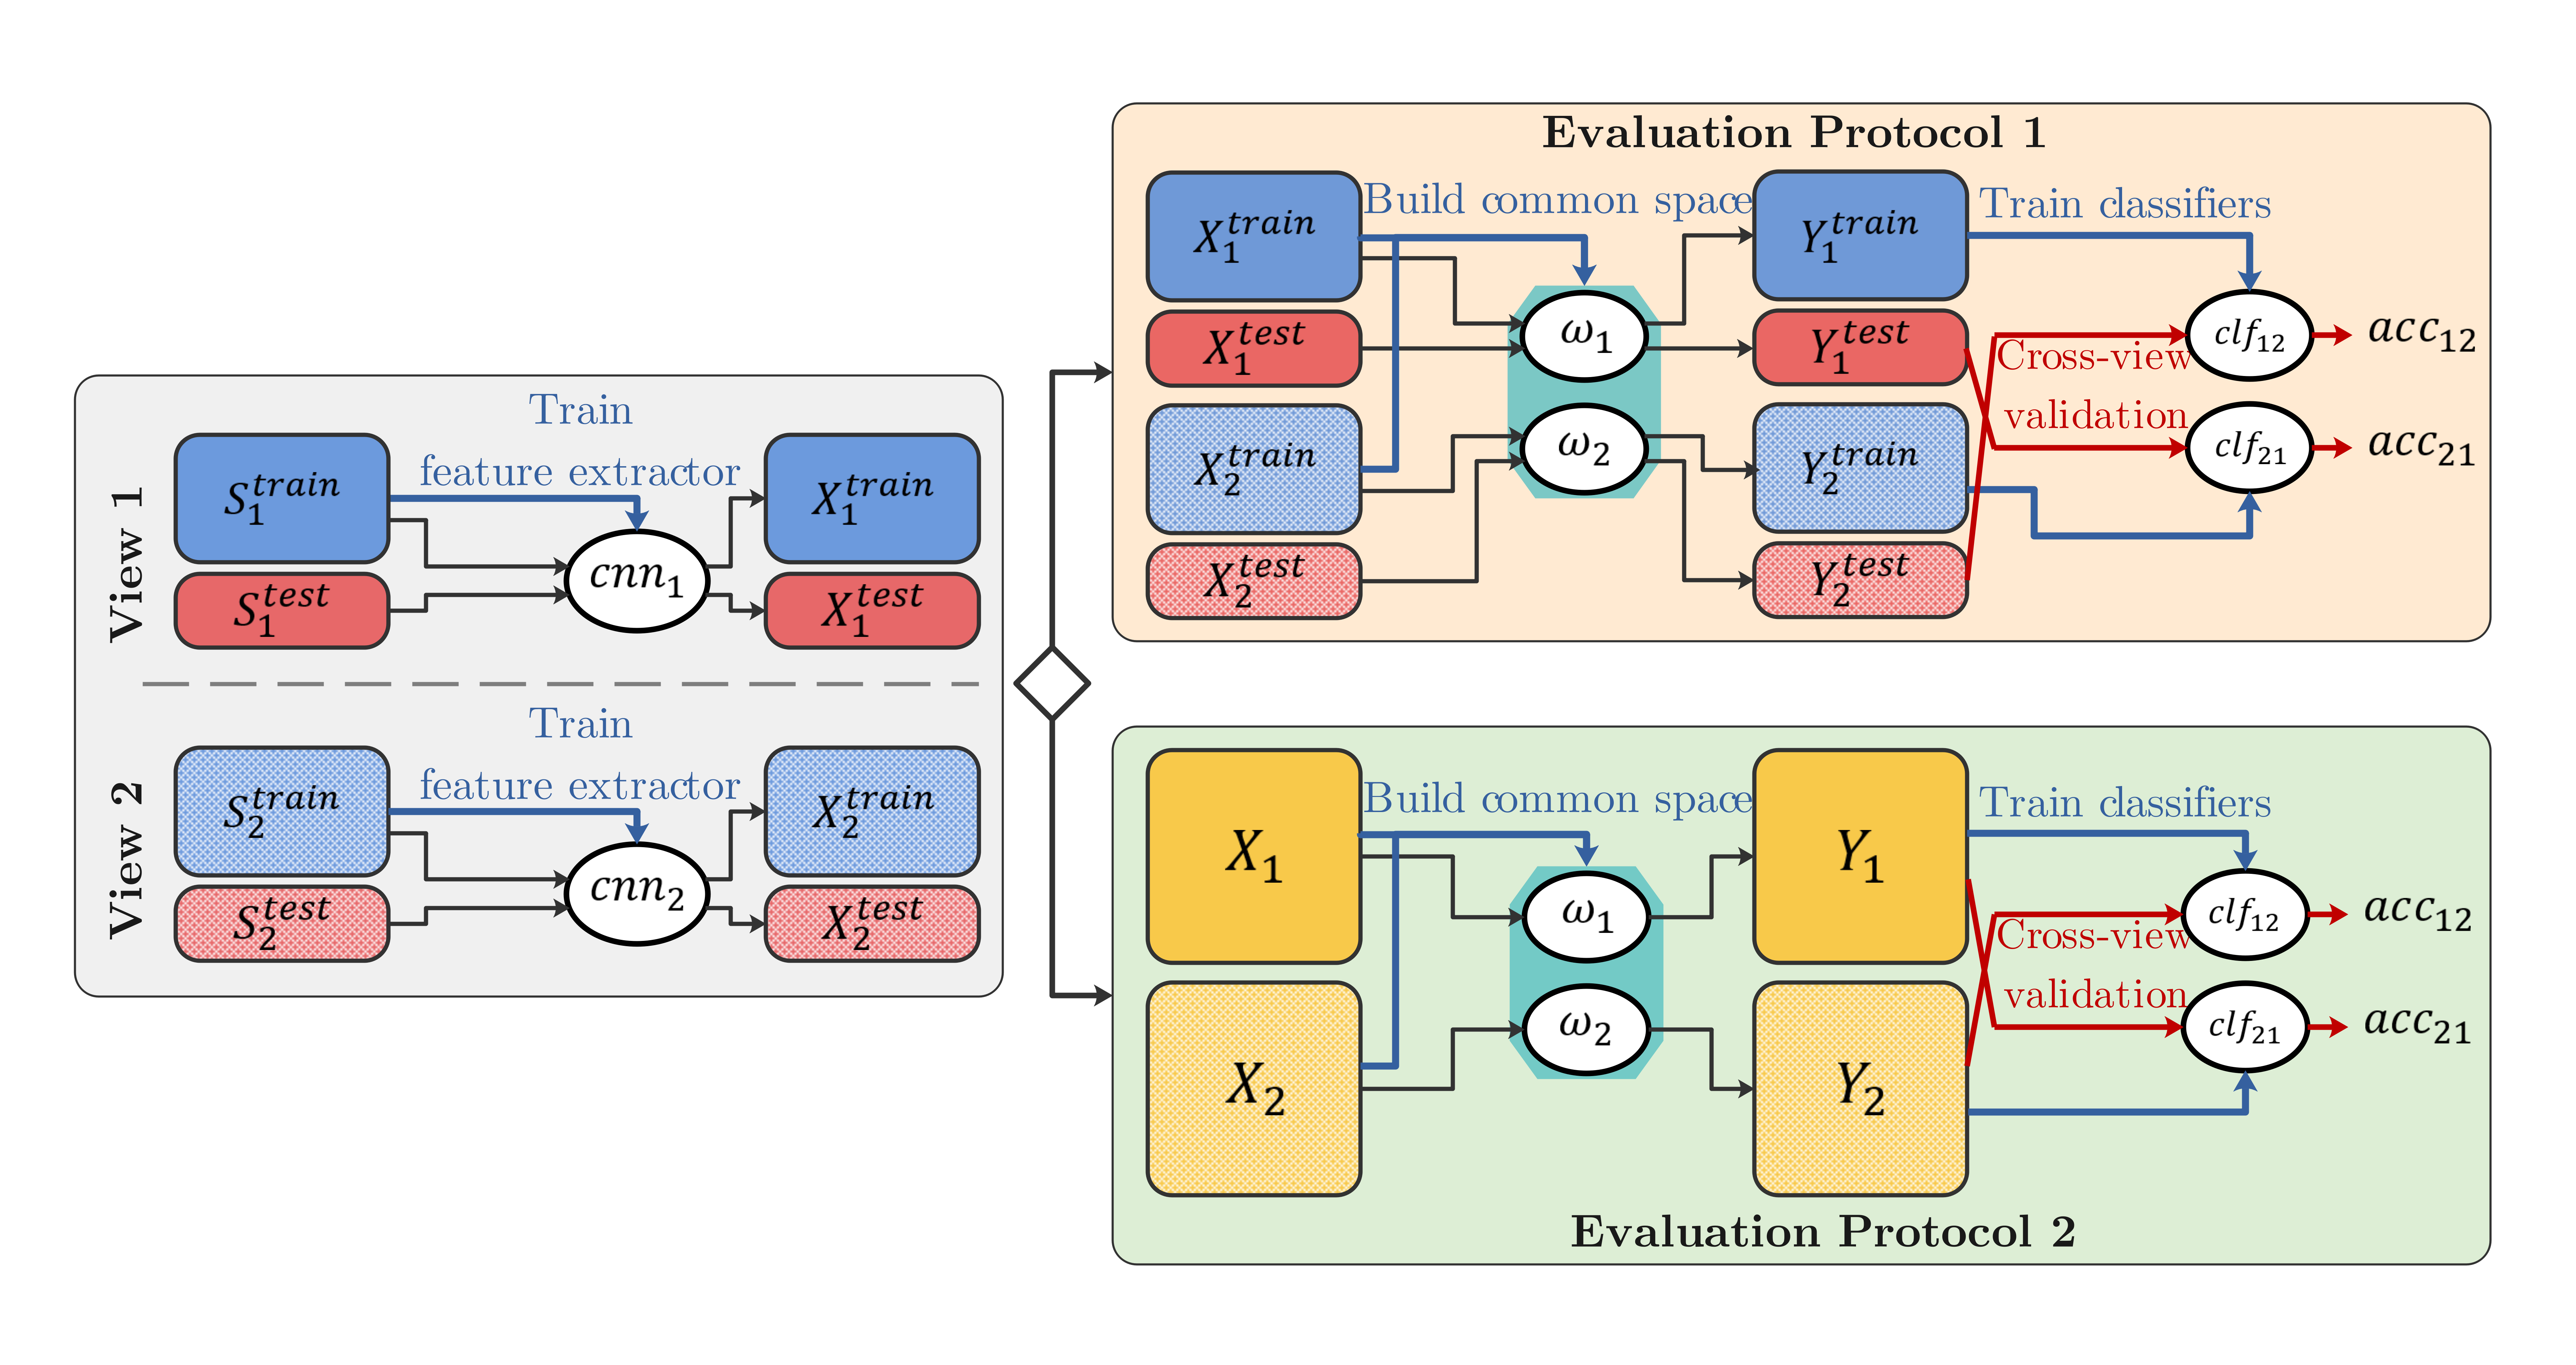
\includegraphics[width=1\linewidth]{figs/protocol.png}
      \caption{Two evaluation protocols used in experiments.}
        %\vspace{-0.3cm}
      \label{Fig:ep}
    \end{figure}
    The overall cross-view evaluation score is computed as average of all evaluation scores of each split, whose method of computation is described specifically in Figure \ref{Fig:ep}:
    \begin{equation}
        {acc}_{ij} = \frac{\sum_{k=1}^M {acc}^{(k)}_{ij}}{M}
    \end{equation}
    where M is the number of actors. Both protocols finally generate a cross-view accuracy matrix as follows:
    \begin{equation}
        \left[\begin{matrix}{acc}_{11}&{acc}_{12}&\cdots&{acc}_{1v}\\{acc}_{21}&{acc}_{22}&\cdots&{acc}_{2v}\\\vdots&\vdots&\ddots&\vdots\\{acc}_{v1}&{acc}_{v2}&\cdots&{acc}_{vv}\\\end{matrix}\right]
        \label{eq:multi-view_scores}
    \end{equation}
    For eager expression, let's define function $\operatorname{accuracy}\left(Y, \tilde{Y}\right)$ as the accuracy score when fitting a classifier on $Y$ features and evaluating its prediction on $\tilde{Y}$ features. Each cell can be expressed accordingly:
    \begin{align}
        {score}_{jr}^{\boldsymbol{protocol 1}} & =\left<\left\{\operatorname{accuracy}\left(Y_j^{train},Y_r^{test}\right)\middle|\ j,r=(1,..,v)\right\}\right> \\
        {score}_{jr}^{\boldsymbol{protocol 2}} & =\left<\left\{\operatorname{accuracy}\left(Y_j,Y_r\right)\middle|\ j,r=(1,..,v)\right\}\right>
    \end{align}

    \textbf{Multi-view strategy:} As MvDA and its variants can theoretically scale for an arbitrary number of views, in order to fairly compare the proposed algorithm with others that only apply for 2 views, we also experiment 2 different multi-view strategies. The key idea is that each strategy restricts the number of views participated in the training process of MvA algorithms.

    In ``\emph{multi-view}'' strategy, only one set of $W^*=\left\{{\omega}_1, {\omega}_2, ..., {\omega}_v\right\}$ is learnt and all separated view features are transformed $Y_j=\omega_j^TX_j,\ j=(1,...,v)$ before computation of accuracy.

    In ``\emph{cross-view}'' strategy, each cell ${score}_{jr}$ of \eqref{eq:multi-view_scores} must be calculated exclusively with the inclusion of only features of those views $j$ and $r$ (wihtout information from other views).
    Therefore, for each distinct combination $jk$, $W_{jr}^*=\left\{{\omega}_j, {\omega}_r\right\}$ is learnt to transform $X_j$ and $X_r$. The diagonal of \eqref{eq:multi-view_scores} is also ignored in this strategy.

    Since there are many scores generated by such extra complicated cross validation process when cycling through every actors, the final reported is average of all.
    Further, it is noticed that in existing works, the evaluation have been done mostly similar to the second evaluation protocol. Hence, in comparison with state of the art techniques, only the scores resulted from the second evaluation protocol are taken.

    %!TEX root = ../../main.tex

\section{Experimental Setup} \label{sec:experimental_setup}
    \subsection{Programming Environment and Libraries}
        The majority of the code implementation is written in Python, fueled by PyTorch \cite{NEURIPS2019_9015} deep learning framework.
        The framework offers powerful supports for matrix manipulation, automatic diffirentiation, accelerated training of deep neural networks on parallel computing platforms and flexibility to efficiently research new algorithmic approaches.
        The MvDA and MvDA-vc Matlab implementations are inherited from the repository published by \cite{kan2015multi} with slight modifications.
        The implementation of proposed pc-MvDA is published at \github{https://github.com/inspiros/pcmvda}.

    \subsection{Configurations}
        \paragraph{Feature extractors}
        All models are trained for 60 epoches with SGD optimizer, initial learning rate is 0.0003 and momentum is 0.9.
        The choosen pre-trained models are:
        \begin{itemize}
            \item{ResNet-50} model was pre-trained on ImageNet dataset and is available in subpackage \textit{torchvision.models} of PyTorch.
            \item{C3D} model was pre-trained on Sports-1M \cite{karpathy2014large} then fine-tuned on Kinetics dataset \cite{kay2017kinetics}. The model is implemented by \cite{VMZ} in Caffe2 deep learning framework, which was improved from original model presented in \cite{tran2015learning} by inserting Batch Normalization layers after each Convolution layer.
            \item{ResNet-50 3D} was pre-trained on Kinetics dataset and weights are given by \cite{hara2018can}.
        \end{itemize}

        \paragraph{Multi-view analysis algorithms}
        Output dimensions of both algorithms are 200. MvDA has no alterable parameter and $\lambda$ of view-consistency term in MvDA-vc is set to 0.03.
        For pc-MvDA, the hyperparameters are $\beta = 1$ and $q = 1$ and the optimizer utilized is Adam with initial learning rate set to 0.01, on each experiment trained 300 epochs.

        \paragraph{Classifier}
        For comparison with related methods, the final classifier used is kNN with $k = 1$.

    %!TEX root = ../../../main.tex

\section{Experimental Results and Discussions} \label{sec:results}
    %!TEX root = ../../../main.tex

\subsection{Experimental results on IXMAS dataset}
    \paragraph{1) Cross-view validation:} In this experiment, we train on data from one view (training view) and testing on data from another view (testing view) then compute the accuracies for two evaluation protocols. Table \ref{tab:cross_p1_ixmas} shows comparative results of using different deep features (C3D, ResNet-50 3D, ResNet-50 RNN, ResNet-50 TA, ResNet-50 AP) and multi-view discriminant analysis techniques (MvDA, MvDA-vc and our proposed pc-MvDA). 

    With the first evaluation protocol, the proposed pc-MvDA, when combined with deep features, gives mostly best accuracy for both evaluation protocols. With C3D features, accuracy by pc-MvDA (88.43\%) is 6.6\% higher than MvDA (81.84\%). pc-MvDA is even better than MvDA-vc (2.87\%). pc-MvDA achieved higher accuracy (about 6\% higher) than MvDA and MvDA-vc with ResNet-50 TA and ResNet-50 AP features. In average, pc-MvDA is 3.09\% higher than MvDA and 1.4\% higher than MvDA-vc.
    
    \begin{table}[htbp]
    \centering
    \caption{Cross-view recognition comparison on IXMAS dataset.}
    \resizebox{0.8\textwidth}{!}{
    \begin{tabular}{|l|c|c|c|c|c|c|}
        \hline
        \multirow{2}{*}{Deep features}          & \multicolumn{3}{c|}{Protocol 1}   & \multicolumn{3}{c|}{Protocol 2}           \\ \cline{2-7} 
                                                & MvDA  & MvDA-vc & pc-MvDA         & MvDA  & MvDA-vc        & pc-MvDA          \\ \hline
        \multicolumn{1}{|c|}{C3D}               & 81.84 & 85.56   & \textbf{88.43}  & 96.54 & 99.29          & \textbf{99.98}   \\ \hline
        \multicolumn{1}{|c|}{ResNet-50 3D}      & 91.25 & 92.19   & \textbf{92.89}  & 97.30 & \textbf{99.73} & 99.65            \\ \hline
        \multicolumn{1}{|c|}{ResNet-50 RNN}     & 75.51 & 76.12   & \textbf{76.54}  & 99.99 & 99.71          & \textbf{100}     \\ \hline
        \multicolumn{1}{|c|}{ResNet-50 TA}      & 79.44 & 80.58   & \textbf{82.05}  & 99.33 & 99.34          & \textbf{99.84}   \\ \hline
        \multicolumn{1}{|c|}{ResNet-50 AP}      & 77.00 & 79.04   & \textbf{80.58}  & 99.68 & 99.81          & \textbf{99.92}   \\ \hline
    \end{tabular}}
    \label{tab:cross_p1_ixmas}
    \end{table}

    For the second evaluation protocol, pc-MvDA almost always keeps better performance compared to MvDA and MvDA-vc. The recognition accuracy scores obtained by both pc-MvDA and MvDA-vc are nearly 100\% for every kind of deep features. With C3D features and ResNet-50 3D features, pc-MvDA is 99.98\% and 99.65\%, which is 3.44\% and 2.35\% higher than the orginal MvDA (96.54\% and 97.3\%) respectively. In average, pc-MvDA is 1.31\% better than MvDA and 0.3\% better than MvDA-vc. 

    In terms of deep features, with the first evaluation protocol, ResNet-50 3D gives the best accuracy (92.89\%) following by C3D (88.43\%), ResNet-50 TA (82.05\%), ResNet-50 AP (80.58\%). The lowest accuracy obtained by ResNet-50 RNN is only 76.54\%. It shows that ResNet-50 3D produces the most discriminative feature space. %Table \ref{tab:cross_feature_ixmas} shows comparative results when using pc-MvDA method with different deep features regarding pairwise views. 

    \begin{table}[htbp]
    \centering
    \caption{Cross-view recognition results of different features on IXMAS dataset with pc-MvDA method. The result in the bracket are accuracies of using features C3D, ResNet-50 3D, ResNet-50 RNN, ResNet-50 TA, Restnet-50 AP respectively. Each row corresponds to training view (from view C0 to view C3). Each column corresponds to testing view (from view C0 to view C3).}
    \resizebox{\textwidth}{!}{\begin{tabular}{|c|c|c|c|c|}
        \hline
        \backslashbox{Training}{Testing} & C0 & C1 & C2 & C3 \\ \hline
        C0 & N/A & (90.7, \textbf{91.9}, 81.6, 84.6, 83.6) & (86.9, \textbf{93.9}, 78.0, 79.6, 78.1) & (89.9, \textbf{93.4}, 76.3, 82.8, 82.1) \\ \hline
        C1 & (86.6, \textbf{91.9}, 71.5, 81.1, 77.5) & N/A & (85.9, \textbf{94.2}, 78.6, 79.3, 80.3) & (88.9, \textbf{93.7}, 74.8, 82.3, 81.3) \\ \hline
        C2 & (87.6, \textbf{92.4}, 72.8, 81.8, 78.5) & (90.7, \textbf{91.7}, 80.6, 83.6, 82.6) & N/A & (89.4, \textbf{93.7}, 75.5, 82.3, 80.6) \\ \hline
        C3 & (87.6, \textbf{92.9}, 70.2, 82.1, 78.8) & (90.7, \textbf{91.2}, 81.6, 84.1, 82.8) & (86.4, \textbf{93.7}, 77.3, 80.6, 80.8) & N/A \\ \hline
    \end{tabular}}
    \label{tab:cross_feature_ixmas}
    \end{table}

    \paragraph{2) Multi-view validation} Table \ref{tab:ixmas_multi} shows multi-view recognition results. The conclusion is consistent with the case of cross-view evaluation: ResNet-50 3D is the best feature extractor. When it is combined with pc-MvDA, the framework gives the highest accuracy for the first protocol (92.82\%), following by C3D (88.19\%), ResNet-50 TA (81.49\%), ResNet-50 AP(80.43\%), and ResNet-50 RNN (76.47\%). Both MvA algorithms give similar accuracies for the second evaluation protocols (nearly 100\%). Again, pc-MvDA enhances the performance of MvDA by 2.43\% for the first protocol and 0.83\% for the second protocol. It only gives slightly better result than MvDA-vc (0.83\% for the first protocol and 0.74\% for the second protocol). 

    \begin{table}[htbp]
    \centering
    \caption{Multi-view recognition comparison on IXMAS dataset.}
    \resizebox{0.7\textwidth}{!}{\begin{tabular}{|c|c|c|c|c|c|c|}
        \hline
        \multirow{2}{*}{Deep features}          & \multicolumn{3}{c|}{Protocol 1}   & \multicolumn{3}{c|}{Protocol2}                    \\ \cline{2-7} 
                                                & MvDA  & MvDA-vc & pc-MvDA         & MvDA           & MvDA-vc        & pc-MvDA         \\ \hline
        \multicolumn{1}{|c|}{C3D}               & 86.93 & 87.04   & \textbf{88.19}  & \textbf{99.99} & 99.44          & \textbf{99.98}  \\ \hline
        \multicolumn{1}{|c|}{ResNet-50 3D}      & 91.84 & 92.33   & \textbf{92.82}  & \textbf{100}   & 99.80          & 99,67           \\ \hline
        \multicolumn{1}{|c|}{ResNet-50 RNN}     & 72.44 & 75.95   & \textbf{76.47}  & 99.34          & \textbf{99.97} & \textbf{99.96}  \\ \hline
        \multicolumn{1}{|c|}{ResNet-50 TA}      & 76.74 & 81.01   & \textbf{81.49}  & 95.80          & 98.25          & \textbf{99.79}  \\ \hline
        \multicolumn{1}{|c|}{ResNet-50 AP}      & 79.28 & 78.93   & \textbf{80.43}  & \textbf{100}   & 98.11          & 99.85           \\ \hline
    \end{tabular}}
    \label{tab:ixmas_multi}
    \end{table}

    Figure \ref{fig:pc-MvDA_confusion_ixmas} compares the performance of feature extractors regarding each action class in multi-view evaluation scheme combined with the first evaluation protocol. There are clear margins between the performance of ResNet-50 3D and followed by C3D with other types of deep features, especially in harder actions (the first class to the third class and the eighth class to the eleventh class). These actions (check watch, cross arm, scratch head, wave, punch, kick, point) involve the most part static pose of the body and only movement of limbs, whereas other actions 4 - sit down, 5 - get up, 6 - turn around, 7 - walk and 12 - pickup include movement of the whole body and are easier to be recognized. This suggests that 3D convolution can better deal with small difference of movement in action images, which in turn generates a much more classification-ready feature space for latter stage of recognition.

    \begin{figure}[htbp]
        \centering
        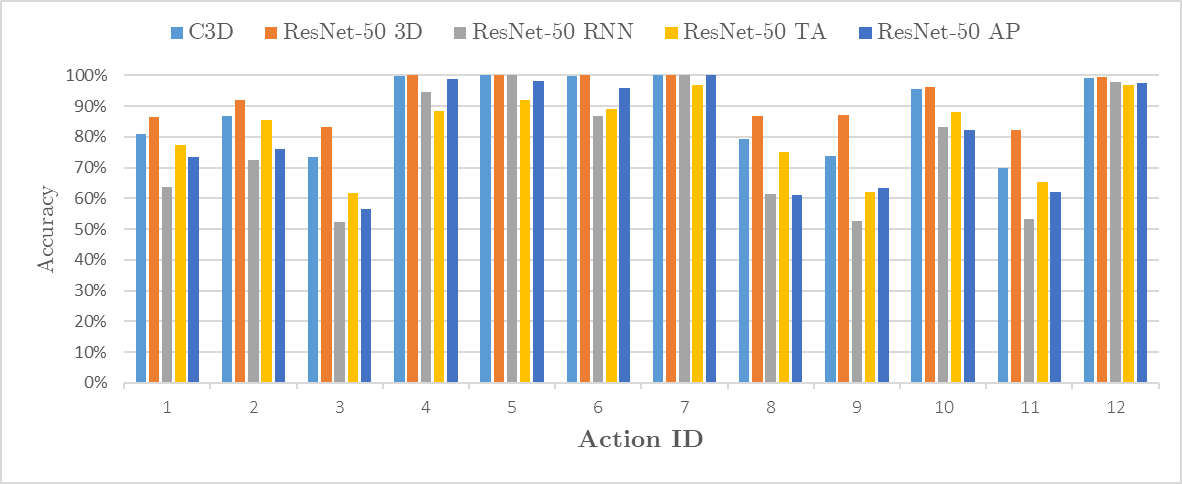
\includegraphics[width=0.8\linewidth]{figs/pc-MvDA_confusion_ixmas.png}
        \caption{Comparison of accuracy on each action class using different deep features combined with pc-MvDA on IXMAS dataset.}
        %\vspace{-0.3cm}
        \label{fig:pc-MvDA_confusion_ixmas}
    \end{figure}

    Table \ref{tab:sota_ixmas} compares the best combination of ResNet-50 3D and pc-MvDA with state-of-the-art frameworks. The comparison is for reference only because in other works, low-level hand-crafted video representation is used as private features and train-test strategy is leave-one-class out, which is not applicable to supervised deep feature extractors in this work. However, the results are still commensurable. % in circumstances where supervised approaches are adopted.
    % TODO - High priority

    \begin{table}[htbp]
    \centering
    \caption{Comparison of proposed methods with SOTA methods on IXMAS dataset according to the second evaluation protocol.}
    \resizebox{0.7\textwidth}{!}{
    \begin{tabular}{|c|c|c|}
    \hline
    Methods                                                              & Cross-view & Multi-view \\ \hline
    Liu et al. \cite{liu2011cross}                                   & 76.32      & N/A       \\ \hline
    Zheng et al. \cite{zheng2012cross}                               & 95.1       & 99.32     \\ \hline
    Zheng et al. \cite{zheng2016cross}                               & 97.8       & 99.4      \\ \hline
    Kong et al. \cite{kong2017deeply}                                & 99.92      & 100       \\ \hline
    Ulhaq et al. \cite{ulhaq2017space}                               & 66.82      & 92.47     \\ \hline
    Zhang et al. \cite{zhang2018cross}                               & 84.1       & N/A        \\ \hline
    Liu et al. \cite{liu2018learning}                                & N/A        & 90.3     \\ \hline
    Liu et al. \cite{liu2018hierarchically}                          & 99.95      & 99.67     \\ \hline
    Proposed method (ResNet-50 3D + pc-MvDA)                     & 99.67      & 99.65       \\ \hline
    \end{tabular}}
    \label{tab:sota_ixmas}
    \end{table}

    %!TEX root = ../../../main.tex

\subsection{Experimental results on MuHAVi dataset}
    \paragraph{1) Cross-view validation:} Table.\ref{tab:muhavi_cross} illustrates cross-view recognition results. The proposed pc-MvDA consistently produces a better average accuracy of around 96.19\% for protocol 1, approximately 4.55\% and 1.51\% higher than that of MvDA (91.64\%) and MvDA-vc (94.67\%) respectively.

    \begin{table}[htbp]
    \centering
    \caption{Cross-view recognition comparison on MuHAVi dataset.}
    \resizebox{0.8\textwidth}{!}{
    \begin{tabular}{|c|c|c|c|c|c|c|}
        \hline
        \multirow{2}{*}{Deep features}          & \multicolumn{3}{c|}{Protocol 1}   & \multicolumn{3}{c|}{Protocol 2}           \\ \cline{2-7} 
                                                & MvDA  & MvDA-vc & pc-MvDA         & MvDA  & MvDA-vc        & pc-MvDA          \\ \hline
        \multicolumn{1}{|c|}{C3D}               & 92.85 & 95.15   & \textbf{97.65}  & 98.95 & 99.76          & \textbf{100}     \\ \hline
        \multicolumn{1}{|c|}{ResNet-50 3D}      & 97.94 & 99.15   & \textbf{99.18}  & 96.77 & \textbf{99.94} & \textbf{99.94}   \\ \hline
        \multicolumn{1}{|c|}{ResNet-50 RNN}     & 95.54 & 95.14   & \textbf{96.18}  & 98.70 & 99.05          & \textbf{99.99}   \\ \hline
        \multicolumn{1}{|c|}{ResNet-50 TA}      & 85.80 & 88.95   & \textbf{91.12}  & 96.57 & 97.03          & \textbf{99.88}   \\ \hline
        \multicolumn{1}{|c|}{ResNet-50 AP}      & 86.09 & 94.98   & \textbf{96.82}  & 89.04 & 98.62          & \textbf{99.93}   \\ \hline
    \end{tabular}}
    \label{tab:muhavi_cross}
    \end{table}

    %Results in Table.\ref{tab:cross_feature_muhavi} show that our combination with ResNet-50 3D has the highest accuracies in almost every circumstances, even though both features coupled with our proposed pc-MvDA give satisfactory performance with all scores exceeding 91\%.

    \begin{table}[htbp]
    \centering
    \caption{Cross-view recognition results of different features on MuHAVi dataset with pc-MvDA method. The result in the bracket are accuracies of using features C3D, ResNet-50 3D, ResNet-50 RNN, ResNet-50 TA, ResNet-50 AP respectively. Each row corresponds to training view (from view C1 to view C7). Each column corresponds to testing view (from view C1 to view C7).}
    \resizebox{\textwidth}{!}{\begin{tabular}{|c|c|c|c|c|c|c|c|}
        \hline
        \backslashbox{Training}{Testing} & C1 & C2 & C3 & C4 & C5 & C6 & C7 \\ \hline
        C1 & N/A & \begin{tabular}{@{}c@{}} (96.1, \textbf{100}, 96.8, \\ 88.5, 98.5) \end{tabular} & \begin{tabular}{@{}c@{}} (98.6, \textbf{99.6}, 96.6, \\ 88.9, 96.3) \end{tabular} & \begin{tabular}{@{}c@{}} (98.6, \textbf{99.6}, 98.0, \\ 93.1, 98.2) \end{tabular} & \begin{tabular}{@{}c@{}} (97.7, \textbf{99.6}, 95.4, \\ 91.3, 96.1) \end{tabular} & \begin{tabular}{@{}c@{}} (97.7, \textbf{98.4}, 92.3, \\ 93.1, 96.3) \end{tabular} & \begin{tabular}{@{}c@{}} (98.2, \textbf{98.5}, 97.2, \\ 89.8, 97.1) \end{tabular} \\ \hline
        C2 & \begin{tabular}{@{}c@{}} (95.6, \textbf{99.0}, 95.2, \\ 91.3, 95.5) \end{tabular} & N/A & \begin{tabular}{@{}c@{}} (98.9, \textbf{99.6}, 96.9, \\ 90.3, 96.1) \end{tabular} & \begin{tabular}{@{}c@{}} (98.4, \textbf{99.6}, 97.6, \\ 92.6, 98.2) \end{tabular} & \begin{tabular}{@{}c@{}} (97.7, \textbf{99.6}, 95.4, \\ 90.9, 96.1) \end{tabular} & \begin{tabular}{@{}c@{}} (97.8, \textbf{98.4}, 92.7, \\ 93.6, 96.5) \end{tabular} & \begin{tabular}{@{}c@{}} (98.6, \textbf{99.0}, 97.4, \\ 90.6, 96.9) \end{tabular} \\ \hline
        C3 & \begin{tabular}{@{}c@{}} (96.1, \textbf{99.0}, 95.6, \\ 90.3, 95.1) \end{tabular} & \begin{tabular}{@{}c@{}} (97.0, \textbf{100}, 96.7, \\ 88.4, 97.8) \end{tabular} & N/A & \begin{tabular}{@{}c@{}} (98.1, \textbf{99.2}, 98.2, \\ 92.8, 98.2) \end{tabular} & \begin{tabular}{@{}c@{}} (97.9, \textbf{99.6}, 95.4, \\ 90.2, 95.6) \end{tabular} & \begin{tabular}{@{}c@{}} (97.9, \textbf{98.2}, 93.0, \\ 94.2, 96.5) \end{tabular} & \begin{tabular}{@{}c@{}} (97.8, \textbf{98.7}, 97.4, \\ 89.4, 97.6) \end{tabular} \\ \hline
        C4 & \begin{tabular}{@{}c@{}} (96.4, \textbf{98.8}, 95.4, \\ 89.6, 95.3) \end{tabular} & \begin{tabular}{@{}c@{}} (96.3, \textbf{100}, 96.6, \\ 91.0, 98.5) \end{tabular} & \begin{tabular}{@{}c@{}} (98.6, \textbf{99.6}, 97.3, \\ 89.5, 96.1) \end{tabular} & N/A & \begin{tabular}{@{}c@{}} (97.7, \textbf{99.4}, 95.6, \\ 91.3, 96.1) \end{tabular} & \begin{tabular}{@{}c@{}} (\textbf{98.4}, 98.0, 93.2, \\ 93.8, 95.6) \end{tabular} & \begin{tabular}{@{}c@{}} (97.7, \textbf{98.7}, 97.4, \\ 91.3, 96.7) \end{tabular} \\ \hline
        C5 & \begin{tabular}{@{}c@{}} (95.9, \textbf{99.0}, 95.6, \\ 91.3, 95.5) \end{tabular} & \begin{tabular}{@{}c@{}} (96.6, \textbf{100}, 97.1, \\ 89.9, 98.3) \end{tabular} & \begin{tabular}{@{}c@{}} (98.8, \textbf{99.4}, 96.8, \\ 90.7, 96.1) \end{tabular} & \begin{tabular}{@{}c@{}} (98.4, \textbf{99.6}, 98.0, \\ 92.1, 97.6) \end{tabular} & N/A & \begin{tabular}{@{}c@{}} (97.9, \textbf{98.2}, 93.4, \\ 94.4, 96.8) \end{tabular} & \begin{tabular}{@{}c@{}} (98.0, \textbf{98.7}, 96.9, \\ 89.0, 97.8) \end{tabular} \\ \hline
        C6 & \begin{tabular}{@{}c@{}} (95.8, \textbf{99.0}, 95.8, \\ 90.3, 95.0) \end{tabular} & \begin{tabular}{@{}c@{}} (97.0, \textbf{100}, 97.6, \\ 89.7, 98.5) \end{tabular} & \begin{tabular}{@{}c@{}} (98.8, \textbf{99.6}, 96.9, \\ 88.7, 96.1) \end{tabular} & \begin{tabular}{@{}c@{}} (98.4, \textbf{99.4}, 98.0, \\ 92.8, 98.2) \end{tabular} & \begin{tabular}{@{}c@{}} (97.5, \textbf{99.6}, 95.9, \\ 91.2, 95.5) \end{tabular} & N/A & \begin{tabular}{@{}c@{}} (98.2, \textbf{99.0}, 97.2, \\ 90.7, 97.4) \end{tabular} \\ \hline
        C7 & \begin{tabular}{@{}c@{}} (96.2, \textbf{98.8}, 95.7, \\ 91.5, 96.2) \end{tabular} & \begin{tabular}{@{}c@{}} (96.4, \textbf{100}, 97.5, \\ 90.3, 98.5) \end{tabular} & \begin{tabular}{@{}c@{}} (98.4, \textbf{99.0}, 97.3, \\ 90.0, 96.7) \end{tabular} & \begin{tabular}{@{}c@{}} (\textbf{98.8}, 98.8, 98.2, \\ 92.8, 98.0) \end{tabular} & \begin{tabular}{@{}c@{}} (97.5, \textbf{99.8}, 95.9, \\ 91.5, 95.9) \end{tabular} & \begin{tabular}{@{}c@{}} (\textbf{98.9}, 98.2, 92.8, \\ 93.9, 97.1) \end{tabular} & N/A \\ \hline
    \end{tabular}}
    \label{tab:cross_feature_muhavi}
    \end{table}

    \paragraph{2) Multi-view validation}: Table.\ref{tab:muhavi_multi} shows multi-view recognition results. The first protocol shows very close capability of MvDA-vc and pc-MvDA at 95.54\% and 95.83\% whereas MvDA is about 3\% behind at 92.7\%. For the second protocol, our variant exceeds MvDA by 2.21\% and MvDA-vc by 1.49\%. The near perfect results of the second protocol give us the same indication that it is not an inequitable method of comparison of MvA algorithms. 

    \begin{table}[htbp]
    \centering
    \caption{Multi-view recognition comparison on MuHAVi dataset.}
    \resizebox{0.8\textwidth}{!}{
    \begin{tabular}{|c|c|c|c|c|c|c|}
        \hline
        \multirow{2}{*}{Deep features}          & \multicolumn{3}{c|}{Protocol 1}                   & \multicolumn{3}{c|}{Protocol2}            \\ \cline{2-7} 
                                                & MvDA           & MvDA-vc        & pc-MvDA         & MvDA           & MvDA-vc & pc-MvDA        \\ \hline
        \multicolumn{1}{|c|}{C3D}               & 81.80          & 96.05          & \textbf{97.37}  & 88.39          & 99.61   & \textbf{100}   \\ \hline
        \multicolumn{1}{|c|}{ResNet-50 3D}      & 99.07          & 99.12          & \textbf{99.15}  & \textbf{99.98} & 99.96   & 99.89          \\ \hline
        \multicolumn{1}{|c|}{ResNet-50 RNN}     & \textbf{96.18} & 95.55          & 95.97           & \textbf{100}   & 99.00   & 99.98          \\ \hline
        \multicolumn{1}{|c|}{ResNet-50 TA}      & \textbf{90.45} & 89.73          & 90.22           & \textbf{99.92} & 98.17   & 99.72          \\ \hline
        \multicolumn{1}{|c|}{ResNet-50 AP}      & 96.01          & \textbf{96.75} & 96.42           & \textbf{100}   & 95.13   & 99.68          \\ \hline
    \end{tabular}}
    \label{tab:muhavi_multi}
    \end{table}

    Figure \ref{fig:pc-MvDA_confusion_muhavi} compares the performance of feature extractors regarding each action class in multi-view evaluation scheme combined with protocol 1. For this dataset, ResNet-50 3D persistently yields out-standing performance while ResNet-50 TA has the worst recognition rates in all action classes.

    \begin{figure}[htbp]
        \centering
        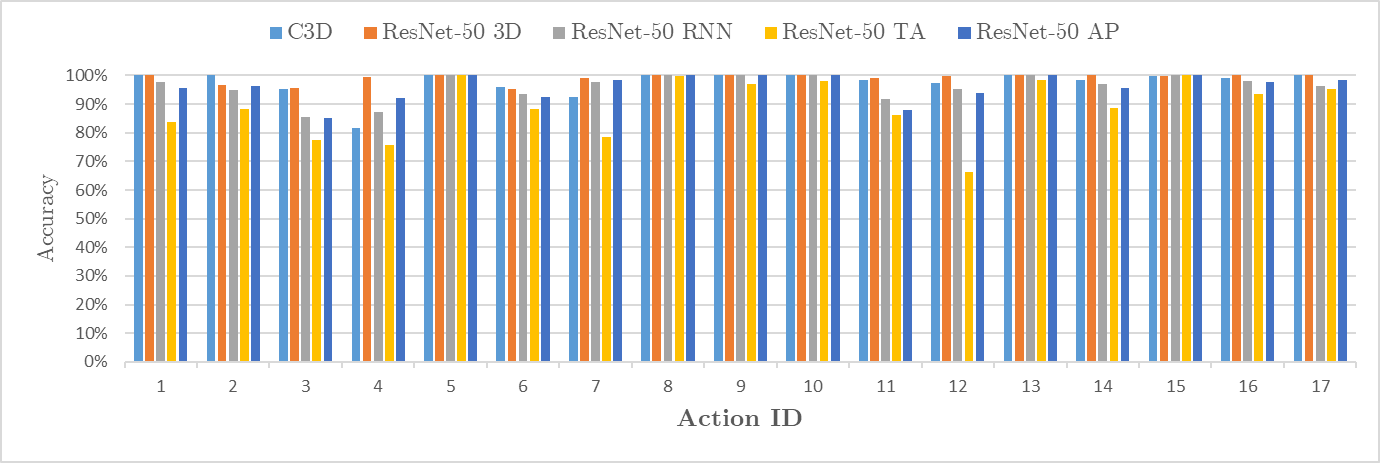
\includegraphics[width=1.0\linewidth]{figs/pc-MvDA_confusion_muhavi.png}
        \caption{Comparison of accuracy on each action class using different deep features combined with pc-MvDA.}
        %\vspace{-0.3cm}
        \label{fig:pc-MvDA_confusion_muhavi}
    \end{figure}

    Table \ref{tab:sota_muhavi} compares the best investigated combination of ResNet-50 3D and pc-MvDA with state-of-the-art frameworks. The comparison is for reference only because of aforementioned difference in setup of number of views and cross validation scheme.

    \begin{table}[htbp]
    \centering
    \caption{Comparison of the proposed methods with SOTA methods on MuHAVi dataset according to the second evaluation protocol.}
    \resizebox{0.7\textwidth}{!}{
    \begin{tabular}{|c|c|c|}
    \hline
    Methods                                                   & Cross-view & Multi-view \\ \hline
    Wu et al. \cite{wu2012view}                               & N/A       & 94.5     \\ \hline
    Zheng et al. \cite{zheng2016cross}                        & 94.88     & 99.8     \\ \hline
    Liu et al. \cite{liu2018learning}                         & N/A       & 91.2     \\ \hline
    Liu et al. \cite{liu2018hierarchically}                   & 99.91     & 99.8     \\ \hline
    Proposed method (ResNet-50 3D + pc-MvDA) \protect\footnotemark              & 99.90     & 99.88    \\ \hline
    \end{tabular}}
    \label{tab:sota_muhavi}
    \end{table}
    \footnotetext{Results when choosing only 4 views Camera 1, Camera 3, Camera 4 and Camera 6 following the other works.}

    %!TEX root = ../../../main.tex

\subsection{Experimental results on MICAGes dataset}

    \paragraph{1) Cross-view validation:} It can be seen in Table.\ref{tab:mica_cross} that pc-MvDA outperforms in almost every cases. With the first protocol, the norm accuracy of pc-MvDA of 74.52\% surpasses that of MvDA-vc (72.12\%) by 2.4\% and that of MvDA (64.94\%) by a large margin of 9.58\%. Especially in case of C3D features, the proposed algorithm achieved 90.2\% recognition rate whereas MvDA returns only 67.13\%.

    \begin{table}[htbp]
    \centering
    \caption{Cross-view recognition comparison on MICAGes dataset.}
    \resizebox{0.8\textwidth}{!}{
    \begin{tabular}{|c|c|c|c|c|c|c|}
        \hline
        \multirow{2}{*}{Deep features}          & \multicolumn{3}{c|}{Protocol 1}          & \multicolumn{3}{c|}{Protocol 2}            \\ \cline{2-7} 
                                                & MvDA  & MvDA-vc        & pc-MvDA         & MvDA  & MvDA-vc        & pc-MvDA           \\ \hline
        \multicolumn{1}{|c|}{C3D}               & 67.13 & 85.98          & \textbf{90.20}  & 93.74 & 99.80          & \textbf{100}      \\ \hline
        \multicolumn{1}{|c|}{ResNet-50 3D}      & 94.91 & 95.25          & \textbf{95.62}  & 97.43 & \textbf{99.97} & 99.79             \\ \hline
        \multicolumn{1}{|c|}{ResNet-50 RNN}     & 58.01 & 61.64          & \textbf{64.13}  & 100   & 100            & 100               \\ \hline
        \multicolumn{1}{|c|}{ResNet-50 TA}      & 53.58 & \textbf{59.55} & 58.62           & 96.70 & 99.48          & \textbf{99.83}    \\ \hline
        \multicolumn{1}{|c|}{ResNet-50 AP}      & 51.07 & 58.19          & \textbf{64.04}  & 99.73 & \textbf{99.99} & 99.89             \\ \hline
    \end{tabular}}
    \label{tab:mica_cross}
    \end{table}

    %Table.\ref{tab:cross_feature_mica} compares all types of deep features regarding accuracy of the proposed algorithm. 
    The top ranking of features applies identically and radically proves the superiority of 3D convolution based clip-level feature extraction in video recognition: ResNet-50 3D at 95.62\% and C3D at 90.2\%. The rest are ResNet-50 RNN (64.13\%), ResNet-50 AP (64.04\%) and ResNet-50 TA (58.62\%). For the second protocol, MvDA-vc (99.85\%) and pc-MvDA (99.9\%) are nearly even in performance while MvDA achieved 97.52\%.

    \begin{table}[htbp]
    \centering
    \caption{Cross-view recognition results of different features on MICAGes dataset with pc-MvDA method. The result in the bracket are accuracies of using features C3D, ResNet-50 3D, ResNet-50 RNN, ResNet-50 TA, RestNet-50 AP respectively. Each row corresponds to training view (from view K1 to view K5). Each column corresponds to testing view (from view K1 to view K5).}
    \resizebox{\textwidth}{!}{\begin{tabular}{|c|c|c|c|c|c|}
        \hline
        \backslashbox{Training}{Testing} & K1 & K2 & K3 & K4 & K5 \\ \hline
        K1 & N/A & \begin{tabular}{@{}c@{}} (92.9, \textbf{95.5}, 69.4, \\ 63.9, 65.1) \end{tabular} & \begin{tabular}{@{}c@{}} (93.7, \textbf{98.0}, 79.1, \\ 75.8, 74.7) \end{tabular} & \begin{tabular}{@{}c@{}} (90.5, \textbf{97.6}, 64.5, \\ 68.8, 70.8) \end{tabular} & \begin{tabular}{@{}c@{}} (89.2, \textbf{92.6}, 56.0, \\ 43.7, 58.2) \end{tabular} \\ \hline       
        K2 & \begin{tabular}{@{}c@{}} (84.7, \textbf{94.6}, 51.3, \\ 41.4, 53.7) \end{tabular} & N/A & \begin{tabular}{@{}c@{}} (94.6, \textbf{97.6}, 78.9, \\ 75.4, 77.5) \end{tabular} & \begin{tabular}{@{}c@{}} (91.3, \textbf{97.6}, 64.4, \\ 68.5, 68.0) \end{tabular} & \begin{tabular}{@{}c@{}} (87.4, \textbf{92.7}, 56.1, \\ 42.0, 55.6) \end{tabular} \\ \hline       
        K3 & \begin{tabular}{@{}c@{}} (87.5, \textbf{94.9}, 51.9, \\ 43.6, 52.7) \end{tabular} & \begin{tabular}{@{}c@{}} (93.0, \textbf{95.5}, 70.1, \\ 64.7, 63.4) \end{tabular} & N/A & \begin{tabular}{@{}c@{}} (90.0, \textbf{97.6}, 63.2, \\ 62.6, 67.5) \end{tabular} & \begin{tabular}{@{}c@{}} (88.9, \textbf{92.2}, 57.2, \\ 41.8, 56.6) \end{tabular} \\ \hline       
        K4 & \begin{tabular}{@{}c@{}} (86.7, \textbf{94.7}, 50.8, \\ 48.9, 54.9) \end{tabular} & \begin{tabular}{@{}c@{}} (90.2, \textbf{95.5}, 71.5, \\ 68.2, 61.8) \end{tabular} & \begin{tabular}{@{}c@{}} (92.5, \textbf{98.0}, 81.0, \\ 76.0, 74.4) \end{tabular} & N/A & \begin{tabular}{@{}c@{}} (89.7, \textbf{92.3}, 54.3, \\ 44.9, 56.6) \end{tabular} \\ \hline       
        K5 & \begin{tabular}{@{}c@{}} (84.9, \textbf{94.9}, 48.4, \\ 41.5, 57.9) \end{tabular} & \begin{tabular}{@{}c@{}} (90.4, \textbf{95.5}, 72.6, \\ 64.1, 65.7) \end{tabular} & \begin{tabular}{@{}c@{}} (94.0, \textbf{97.8}, 79.1, \\ 72.5, 76.3) \end{tabular} & \begin{tabular}{@{}c@{}} (91.9, \textbf{97.3}, 62.7, \\ 64.1, 69.0) \end{tabular} & N/A \\ \hline
    \end{tabular}}
    \label{tab:cross_feature_mica}
    \end{table}

    \paragraph{2) Multi-view validation}: The multi-view recognition results in Table.\ref{tab:mica_multi} shows an almost alike trend for both protocols. In general, pc-MvDA is 8.95\% and 0.72\% higher in accuracy for protocol 1, and 2.75\% and 0.04\% for protocol 2, in comparison with MvDA and MvDA-pc respectively.

    % TODO
    In virtually every experiments of MICAGes and two earlier benchmark datasets, the proposed extension is superior. The average accuracies of pc-MvDA is, in comparison on protocol 1 (and protocol 2 resp.), 5.29\% (1.21\% resp.) higher than MvDA, 1.21\% (0.62\% resp.) better than MvDA-vc. Despite not being as intuitive and straightly intelligible as pairwise-covariance, the multi-view resemblance added in MvDA-vc achieved nearly the performance of pc-MvDA. However, this view-consistency can be easily splitted into pairwise terms and intergrated into the objective of pc-MvDA in future works for further analysis.

    \begin{table}[htbp]
    \centering
    \caption{Multi-view recognition comparison on MICAGes dataset.}
    \resizebox{0.8\textwidth}{!}{
    \begin{tabular}{|c|c|c|c|c|c|c|}
        \hline
        \multirow{2}{*}{Deep features}          & \multicolumn{3}{c|}{Protocol 1}          & \multicolumn{3}{c|}{Protocol2}                     \\ \cline{2-7} 
                                                & MvDA  & MvDA-vc        & pc-MvDA         & MvDA           & MvDA-vc       & pc-MvDA           \\ \hline
        \multicolumn{1}{|c|}{C3D}               & 68.31 & 87.70          & \textbf{89.99}  & 88.79          & 99.54         & \textbf{100}      \\ \hline
        \multicolumn{1}{|c|}{ResNet-50 3D}      & 95.32 & 95.26          & \textbf{95.54}  & \textbf{100}   & 99.96         & 99.80             \\ \hline
        \multicolumn{1}{|c|}{ResNet-50 RNN}     & 57.50 & 63.05          & \textbf{63.83}  & 99.90          & \textbf{100}  & 99.97             \\ \hline
        \multicolumn{1}{|c|}{ResNet-50 TA}      & 54.43 & \textbf{61.46} & 58.25           & 96.72          & 99.49         & \textbf{99.69}    \\ \hline
        \multicolumn{1}{|c|}{ResNet-50 AP}      & 50.93 & 60.20          & \textbf{63.66}  & \textbf{99.99} & 99.93         & 99.67             \\ \hline
    \end{tabular}}
    \label{tab:mica_multi}
    \end{table}

    In addition to the same propensity shown, MICAGes also reveals the robustness of 3D convolution to generate fine clustered private feature space because this dataset contains exclusively hand gestures, which take part in a relatively small region of the captured videos. ResNet-50 3D and C3D are predominant for discriminant common space construction and classification and distances other features (Figure \ref{fig:pc-MvDA_confusion_mica}).

    \begin{figure}[htbp]
        \centering
        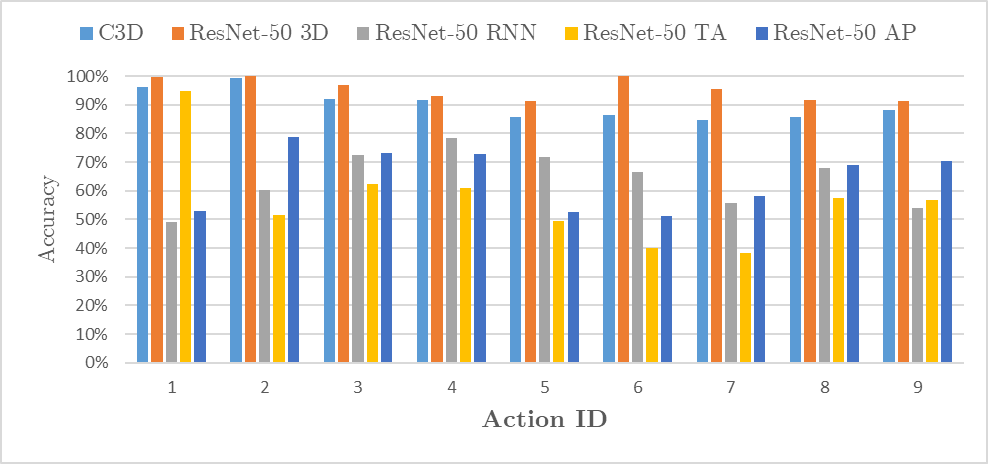
\includegraphics[width=0.8\linewidth]{figs/pc-MvDA_confusion_mica.png}
        \caption{Comparison of accuracy on each action class using different deep features combined with pc-MvDA on MICAGes dataset.}
        %\vspace{-0.3cm}
        \label{fig:pc-MvDA_confusion_mica}
    \end{figure}

    To better study the behavior of investigated multi-view analysis algorithms, t-SNE embedding of original private spaces, MvDA and pc-MvDA common space generated by protocol 1 are plotted in Figure \ref{fig:mica-tsne}. In these scatter plots, colors denote action classes, shapes as different views and train/test data are distinguished by border type. They explicitly denotes the surpassing capability of the proposed algorithm in finding a common space with prominent extra-class discrepancy. The data samples involved in training process are generally clustered in compact and separated blobs while testing data samples dissolve nearby. The better convergence of pc-MvDA compared to the baseline is usually only visible for harder features, whereas with the inputs of ResNet-50 3D features, which are already highly discriminated in private spaces, the improvement of pc-MvDA is negligible. Note that these illustrations of t-SNE embedding do not strictly depict an identical distribution of data.

    \begin{figure}[htbp]
        \centering
        \includegraphics[width=1\linewidth, height=0.6\pdfpageheight, keepaspectratio=false]{figs/mica-tsne.png}
        \caption{First column: private feature spaces stacked and embedded together in a same coordinate system; Second column: MvDA common space; Third column: pc-MvDA common space.}
        %\vspace{-0.3cm}
        \label{fig:mica-tsne}
    \end{figure}



    \section{Summary}
        The experiments conducted indicates that the framework could achieve competitive results.
        The second evaluation protocol is shown to be less equitable for multi-view analysis algorithms compared to the first evaluation protocol represented in this thesis.
        Overall, the proposed pc-MvDA also achieved amelioration in almost every cases compared to baseline MvDA by a 5.29\% margin in terms of average accuracy.
